\chapter{Metodología}
\label{chap:metodologia}

En este capítulo se detallarán el conjunto de procedimientos utilizados para alcanzar los objetivos del proyecto.


\section{Desarrollo  incremental}
Este método consiste en una serie de iteraciones, en pequeñas ventanas de tiempo, en las que al final de las mismas tendremos un producto que el cliente podrá revisar y posteriormente mejorar y/o corregir [Figura~\ref{fig:metodologia}]. 

\begin{figure}[h]
    \centering
    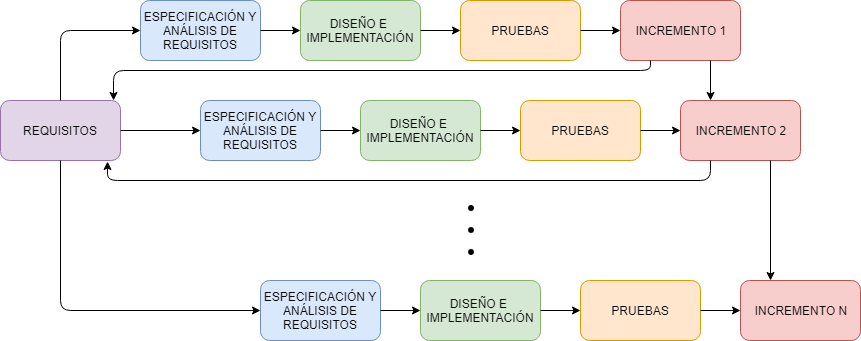
\includegraphics[width=0.8\textwidth, keepaspectratio]{imaxes/Metodologia.png}
    \caption{Fases del modelo incremental}
    \label{fig:metodologia}
\end{figure}

Esta metodología exige tener dos grupos de usuarios:
\begin{itemize}
    \item \textbf{Cliente}: Se encarga de revisar el producto al final de las iteraciones.
    \item \textbf{Desarrollador}: Se encarga de desarrollar el producto.
\end{itemize}

Al ser un proyecto de fin de carrera, no existe un cliente como tal, por lo que se ha decidido que los directores del proyecto tomen el rol de clientes.

Las principales razones por la se ha elegido esta metodología frente a otras existentes son las siguientes:
\begin{enumerate}
    \item \textbf{El cliente no sabe exactamente lo que necesita}: Al inicio del proyecto no se podía prever cómo sería la aplicación, pues debido a la complejidad del proyecto, no se sabía cuál podría ser la mejor manera de hacer que la aplicación para recoger los datos necesarios. 
    
    \item \textbf{Obtener un producto usable rápidamente}: Este proyecto tiene dos etapas claramente diferenciadas, construir una aplicación para recoger datos y analizar esos datos. Claramente la segunda es totalmente dependiente de la primera, por lo que era necesario disponer de un producto usable que permita recopilar información a medida que se amplia su funcionalidad.
    
\end{enumerate}

\section{Iteración 0: Búsqueda de información sobre el dominio}
El objetivo de esta iteración es la búsqueda y recopilación de información sobre el dominio del proyecto. También se definirán los requisitos que el sistema final deberá cumplir, la estructura que se usará para el desarrollo~[Figura~\ref{fig:arquitectura}] y se detallarán los componentes de más bajo nivel~[Figura~\ref{fig:app_schema}]~[Figura~\ref{fig:server_schema}].
De esta forma el desarrollo del proyecto estará bien definido y su implementación debería ser más fácil.

\section{Iteración 1: Sistema de captura de información}
El objetivo de esta fase es la de crear una aplicación que permita capturar la información proveniente del dispositivo. El producto creado al final de esta iteración será una aplicación funcional. El manual de usuario asociado a la aplicación puede consultarse en el Apéndice~\ref{chap:application}.

\subsection{Especificación y análisis de requisitos}
A continuación, se describen los requisitos que la aplicación ha de cumplir:
\begin{itemize}
    \item \textbf{Gestión de los recursos:} Dado que la aplicación recolectará toda la información de los eventos generados por la interacción del usuario con el dispositivo, hay que tener en cuenta cómo manejar dicho volumen de información para evitar el colapso del dispositivo, ya que al tratarse de un \textit{smartphone} o \textit{Tablet}, cuentan con unos recursos limitados tanto en hardware como batería. 
    
     \item \textbf{Formato de los eventos:} Para facilitar el análisis a posteriori la aplicación debe mantener un formato similar en todos los eventos que capture.
     
\end{itemize}


\subsection{Diseño e implementación}
Para realizar la implementación y el diseño de la aplicación se ha usado \textit{Angular} e \textit{Ionic} respectivamente, usando la estructura que se muestra en la Figura~\ref{fig:app_schema}.
 \begin{figure}[h]
    \centering
    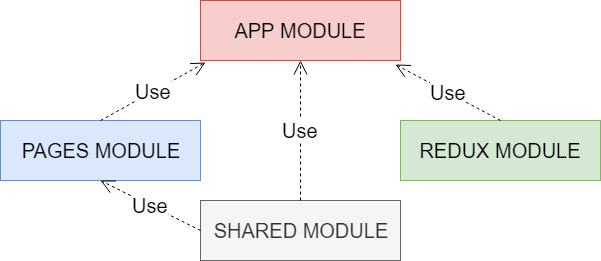
\includegraphics[width=0.8\textwidth, keepaspectratio]{imaxes/APP_SCHEMA.png}
    \caption{Estructura de la aplicación}
    \label{fig:app_schema}
\end{figure}
 
 \subsubsection{App Module}
 Es el módulo principal de la aplicación, en él se encuentra la configuración de los sistemas, y se encarga de hacer de nodo de enlace entre los demás módulos.
 
 
 \subsubsection{Redux Module}
Este módulo implementa toda la lógica del patrón \textit{Redux}. Este patrón permite manejar el estado de la toda aplicación haciendo uso de un objeto central inmutable. Esto permite generar un flujo de datos de una sola dirección y de esta manera que el código sea menos propenso a errores.
 
  \begin{figure}[h]
    \centering
    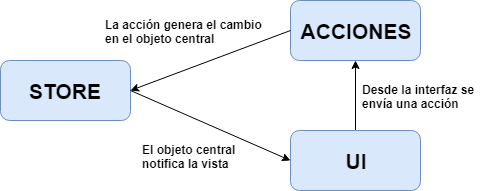
\includegraphics[width=0.8\textwidth, keepaspectratio]{imaxes/redux_simple.png}
    \caption{Ciclo del patrón redux}
    \label{fig:redux_simple}
\end{figure}
 
 \subsubsection{Pages Module}
 Este módulo agrupa al conjunto de ventanas de la aplicación. Cada una de ellas esta implementada en un submódulo. Dicha estructura es implementada por defecto por \textit{Ionic} para poder aplicar la estrategia de carga perezosa (\textit{lazy loading}), la cual solo carga lo que se ve en el momento. Esto permite que la primera carga sea mucho más rápida.
 
 \subsubsection{Shared Module}
 Este módulo contiene los distintos servicios, componentes\dots~ que son reutilizados por varios módulos de la aplicación.
 

\section{Iteración 2: Sistema para el almacenamiento de la información}
En esta fase se pretende crear un servidor que permita el almacenamiento de los eventos recogidos en la primera fase para su posterior análisis. El producto creado al final de esta iteración expone una \textit{API} que se puede consultar en el Apéndice~\ref{chap:rest_api}.

\subsection{Especificación y análisis de requisitos}
A continuación, se describen los requisitos que el servidor ha de cumplir:
\begin{itemize}
    \item \textbf{Gestión de los recursos:} Dado que el servidor ha de permitir el envío y recibo de muchas peticiones por segundo, se ha de tener en cuenta, que el servidor soporte dicha funcionalidad a un coste de recursos bajo.
    
     \item \textbf{Almacenamiento de los eventos:} Dado que la cantidad de eventos que se manejarán será muy alta y con un esquema semi-definido, ya que podría cambiar en un futuro, se necesita una base de datos que sea compatible con estos puntos.
\end{itemize}
\subsection{Diseño e implementación}
 Debido a los requisitos comentados se ha optado por usar Node.js como entorno, por su bajo consumo de recursos. La estructura generada se puede ver en la Figura~\ref{fig:server_schema}.
 
 \begin{figure}[h]
    \centering
    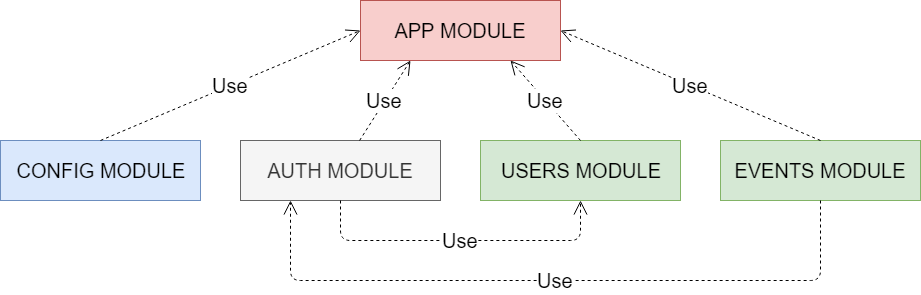
\includegraphics[width=0.8\textwidth, keepaspectratio]{imaxes/server_schema.png}
    \caption{Estructura de la aplicación}
    \label{fig:server_schema}
\end{figure}
 
 \subsubsection{App Module}
 Es el módulo principal desde el cual se llaman a los otros módulos e inicia servicios de terceros, como la conexión con la base datos.
 
 \subsubsection{Config Module}
Este módulo contiene todas las variables externas del sistema, como el puerto, dirección de la base de datos~\dots
 
 \subsubsection{Auth Module}
 En este módulo se realiza la autenticación del usuario, la cual permitirá al usuario realizar ciertas acciones y restringirá otras en función a su rol.
 
  \subsubsection{Users Module}
 En este módulo se encuentra la lógica encargada de procesar la información de los usuarios, como la creación y actualización de estos.
 
 \subsubsection{Events Module}
 En este módulo se encuentra la lógica necesaria para procesar la información relacionada con los eventos que se generan en la aplicación, almacenándolos de forma persistente en la base de datos.

\section{Iteración 3: Comunicar aplicación con servidor}
El objetivo de esta fase es la de comunicar los dos sistemas creados hasta el momento, con el fin de guardar los eventos generados en la primera iteración
      
\subsection{Especificación y análisis de requisitos}
A continuación, se describen los requisitos establecidos para esta iteración:

\begin{itemize}
    \item \textbf{Securizar  conexiones}: Dado que la comunicación se pretende realizar a través de internet usando el protocolo \textit{HTTP 1.1}, es necesario que esta comunicación permanezca cifrado de punto a punto, por lo que usarán los protocolos criptográficos \textit{SSL/TLS}.
    
    \item \textbf{Restringir peticiones}: Algunas peticiones hacia nuestro servidor deberán estar solo disponibles si el usuario cumple ciertas restricciones. Estás peticiones deberán ser realizadas por un usuario administrador.
    
\end{itemize}

\subsection{Diseño e implementación}

Para segurizar toda nuestra aplicación y hacer que esta sea menos propensa a ataques, se ha creado un certificado digital para poder realizar conexiones \textit{HTTPS}.

Para restringir el acceso a nuestro servidor hemos utilizado el estándar \textit{JSON Web Token} (\textit{JWT}), el cual es una cadena de texto codificada que se envía en cada petición. Esta cadena de texto contiene tres partes que contienen la información necesaria para comprobar el usuario y la validez del token.

 \section{Iteración 4: Implementación de la Inteligencia Artificial}
 
 El objetivo de esta iteración es la de tratar los datos obtenidos. Analizando que características obtienen un mejor resultado a la hora de identificar al usuario. Esta iteración se detallará más a fondo en el capítulo \ref{chap:ia}.
 
 \subsection{Especificación y análisis de requisitos}
A continuación, se describen los requisitos establecidos para esta iteración:

\begin{itemize}
    \item \textbf{Obtener un conjunto de datos grande}: Para este tipo de análisis se necesitan  una gran cantidad de datos y representativos de la población. Por lo tanto, es necesario obtener datos de bastantes usuarios de diferentes edades y sexos.
    
    \item \textbf{Obtener características no relacionadas}: Para analizar los eventos, lo ideal es obtener características poco correlacionadas, ya que si estas están correlacionadas estos datos serán redundantes. Es decir, no aportarán ninguna información adicional, pero podrán empeorar los resultados.
\end{itemize}

 \section{Iteración 5: Implementación online de los algoritmos}
 El objetivo de esta iteración es conseguir que el algoritmo entrenado sea accesible en cualquier momento y que su respuesta sea la predicción.
 
 
 \subsection{Especificación y análisis de requisitos}
A continuación, se describen los requisitos establecidos para esta iteración:

\begin{itemize}
    \item \textbf{Integrar los servidores}: Para que el algoritmo no este expuesto directamente en internet, sino que solo sea accesible mediante el servidor principal. De esta manera, la configuración relacionada con la seguridad solo será necesario implementarla en un servidor.
    
    \item \textbf{Gestión de recursos}:  El servidor se encontrará en un maquina física por lo que es necesario controlar que los procedimientos que se lleven a cabo no sean computacionalmente costosos.   
\end{itemize}
 
 \subsection{Diseño e implementación}
 Para conseguir el objetivo de esta iteración se ha creado un servidor en \textit{Python} que permita la ejecución de un conjunto de librerías las cuales usarán el algoritmo entrenado y la respuesta de la petición generada será la predicción hecha por el algoritmo. 

\section{Pruebas}
\label{cap:pruebas}

Las pruebas son las actividades dirigidas a evaluar la capacidad de un programa o sistema y determinar que alcanza los resultados requeridos \cite{hetzel1988complete}.

Existen distintos niveles de pruebas, según se puede observar en la Figura \ref{fig:cohn}, el nivel más bajo pertenecen a las pruebas unitarias, que son las que mayor atención deberemos prestar, seguidas de las pruebas de integración y por último las pruebas \textit{e2e}. 

\begin{figure}[H]
    \centering
    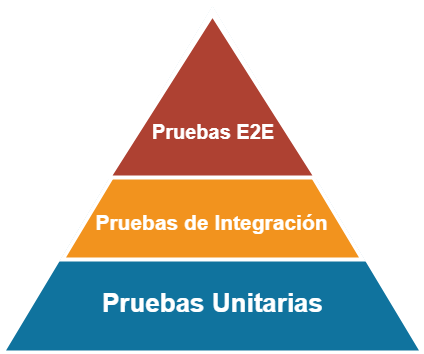
\includegraphics[width=0.5\textwidth]{imaxes/piramide_cohn.png}
    \caption[Pirámide de Cohn]{Pirámide de Cohn \cite{cohn2010succeeding}}
    \label{fig:cohn}
\end{figure}

\subsection{Prueba unitarias}

Estas pruebas son de muy bajo nivel, en ellas se comprueba el correcto funcionamiento de los métodos, clases, componentes\dots

Este tipo de pruebas han sido ejecutadas tanto en el servidor como en la aplicación, para validar el correcto funcionamiento de algunas de las partes más críticas del sistema.

\subsection{Pruebas de integración}

Comprueban el correcto funcionamiento de los componentes una vez integrados. Se ha revisado la integración completa del sistema, validando que todos los módulos funcionasen correctamente.

Este tipo de pruebas han sido ejecutadas en el servidor para validar las rutas creadas. Se han implementado tres bancos de pruebas, cada uno de ellos perteneciente a un módulo de nuestro sistema. En total se han ejecutado doce casos diferentes, y todas han sido satisfactorias [Figura \ref{fig:test_suite_server}]

\begin{figure}[H]
    \centering
    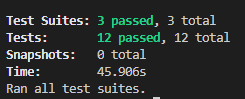
\includegraphics[width=0.5\textwidth]{imaxes/test_suites_server.png}
    \caption{Resultado de las pruebas en el servidor}
    \label{fig:test_suite_server}
\end{figure}

\subsection{Pruebas end to end (e2e)}
Este tipo de pruebas simulan el comportamiento de un usuario real. Prueban toda la aplicación de principio a fin, verificando el correcto funcionamiento de todo el sistema y la navegación entre las distintas ventanas de la aplicación.

\begin{figure}[H]
    \centering
    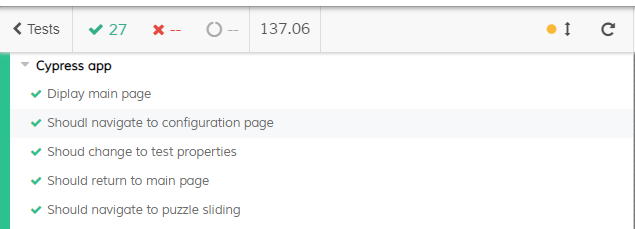
\includegraphics[width=0.7\textwidth]{imaxes/test_suites_app.png}
    \caption[Resultado de las pruebas en la aplicación]{Resultado de las pruebas en la aplicación \cite{cypress_youtube}}
    \label{fig:test_suite_app}
\end{figure}

\subsection{Cobertura}

La cobertura es una medida que nos ayuda a comprobar que partes de nuestro código han sido probadas. Además, sirve para determinar la calidad de la prueba, pues gracias a ella podremos saber que partes del código no hemos comprobado y cuales sí.

\begin{landscape}
    \begin{figure}
        \centering
        
        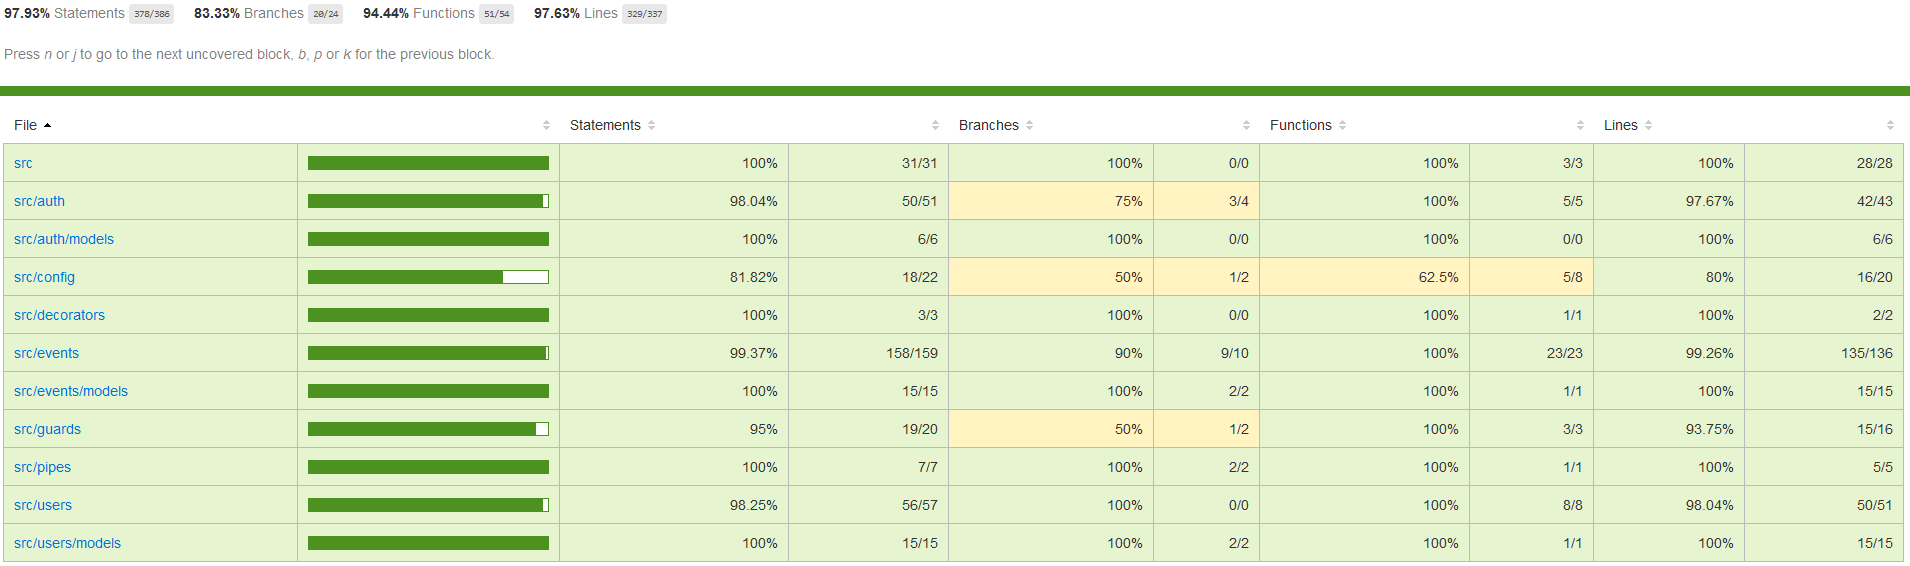
\includegraphics[width=\linewidth,height=0.6\textheight]{imaxes/server_coverage.png}
        \caption{Cobertura de las pruebas del servidor}
        \label{fig:server_coverage}
    \end{figure}
\end{landscape}

